  % Assignment 2
  \question The \emph{bubble-sort} interconnection network $B_4$ is pictured in Fig. 2. In parts ($b$)-($c$), you may assume that $B_4$ is node-symmetric. 
  \begin{parts}
    \part Give an algebraic definition of $B_4$.
    \begin{solution}
      \begin{align*}
        V &= \{(a_1, a_2, a_3, a_4) \in \{1,2,3,4\}^4: a_i \neq a_j \;\forall i = j\}, \\
        E &= \{((a_1, a_2, a_3, a_4), (a_2, a_1, a_3, a_4)): (a_1, a_2, a_3, a_4) \in V\} \;\cup \\
               &\qquad \{((a_1, a_2, a_3, a_4), (a_1, a_3, a_2, a_4)): (a_1, a_2, a_3, a_4) \in V \;\cup \\
               &\qquad \{((a_1, a_2, a_3, a_4), (a_1, a_2, a_4, a_3)): (a_1, a_2, a_3, a_4) \in V\}.
      \end{align*}
    \end{solution}

    \part What is the diameter of $B_4$? You should justify your answer.
    \begin{solution}
      First, we complete a breadth-first search on this graph starting at $4321$ to get the following spanning tree. 
      \begin{center}
% https://tikzcd.yichuanshen.de/#N4Igdg9gJgpgziAXAbVABwnAlgFyxMJZAZgBoAGAXVJADcBDAGwFcYkQAWYgJgEYQAvqXSZc+Qim6le1Ok1bsuvboOEgM2PASJkZNBizaIQxDn1UjN4oh2myDC42eL8hlsdpS9S3e-KOcvDwW6qJaEshSvvr+7KbKIRoeEWTRcoZx3ByuaknhNj5+GcZZLolh1igArIUxxZx8xOVWnsjkpMRFjoHcTW6hLRHenXXdvFwq-XmVkR1dAS5mzck6c6MLfBzL+Si2I+ndvdnbMzX7DgFZQSet7Rzz7OO9N0Ok9+uPppO5Fa1S7wcFsotlNfik3g8SosXgUARd2Js+j9BkQpFVISAglkYSgyOiPiUgiDkStdqR8YDHqUcSRSAA2DHKUyCWQwKAAc3gRFAADMAE4QAC2SHaIBwECQ3hAAAsYPQoEgwMxGIx+vyhSKaOKkFIZXKFYglSq1QLhYhRdrEGQQIx6AAjGCMAAKYPYjBgPJwIBosvliuVqrU6rNUsttj1fsNAZNGsQoYliBqEYNRsDvNNOq1CbpPv1-uNQYzVqzSAA7LnI6mY2brZaABwVlPRwux8OWgCc1aQbYTvHIXcTJbjvAHObFve4o6HQQH5fHko4A7706qS4tvdXLZD68ldKX8clpaXustvDrS57ks7W8PQ+4-Zvcfbd5Hj94z-niG4k8f37vxAESgBCAA
\begin{tikzcd}
     &                                      &                           & 4321 \arrow[ld] \arrow[d] \arrow[rd] &                           &                 \\
     &                                      & 4312 \arrow[ld] \arrow[d] & 3421 \arrow[d]                       & 4231 \arrow[d] \arrow[rd] &                 \\
     & 4132 \arrow[ld] \arrow[d]            & 3412 \arrow[d]            & 3241 \arrow[d] \arrow[rd]            & 2431 \arrow[rd]           & 4213            \\
4123 & 1432 \arrow[ld] \arrow[ld] \arrow[d] & 3142 \arrow[d]            & 3214 \arrow[d]                       & 2341                      & 2413 \arrow[ld] \\
1423 & 1342                                 & 3124 \arrow[d]            & 2314                                 & 2143 \arrow[ld] \arrow[d] &                 \\
     &                                      & 1324                      & 2134                                 & 1243 \arrow[ld]           &                 \\
     &                                      &                           & 1234                                 &                           &                
\end{tikzcd}
    \end{center}
    From this, we assert that a minimum path from $(4,3,2,1)$ to any other node has length at most 6. We now claim this is true for any $y \in V$. Indeed, let $y \in N \setminus \{(4,3,2,1)\}$ and $\sigma: V \to V$ such that $\sigma((4,3,2,1)) = y$ (which exists as $B_4$ is node-symmetric). Now let $z \in V \setminus \{y\}$. Consider the route in the spanning from $(1,2,3,4)$ to $\sigma^{-1}(z)$,
    \[ P = ((4,3,2,1), v_1, \ldots, v_n, \sigma^{-1}(z)) \]
    where $n \leq 4$, and we take the image of this path:
    \[ \sigma(P) = P' = (y, \sigma(v_1), \ldots, \sigma(v_n), z). \]
    As $\sigma$ is an automorphism, this must be a valid path from $y$ to $z$ of length $6$.
    Thus far, we have shown that there always exists a path of size $6$ between any two nodes. We observe that (from our BFS search), there is no path from $(4,3,2,1)$ to $(1,2,3,4)$ that is shorter than $6$. With this, we assert that the diameter of $B_4$ is 6. 
    \end{solution}

    \part Is $B_4$ a moore graph? You should justify your answer.
    \begin{solution}
      $B_4 = (V,E)$ is a moore graph if and only if
      \[ \lvert V \rvert = 1 + d \sum_{i=0}^{k-1} (d-1)^i \]
      where $d$ is the degree of $B_4$ and $k$ is the diameter. From part (b), we have that $k = 6$ and one can reason that $d = 3$. Furthermore, the number of nodes in $B_4$ is just the number of ways you can permute 4 elements, that is $\lvert V \rvert = 4! = 24$.
      We see
      \[ 24 = \lvert V \rvert \neq 1 + d \sum_{i=0}^{k-1} (d-1)^i = 190. \]
      Thus $B_4$ is not moore graph. 
    \end{solution}

    \part Show as many node-disjoint paths as possible joining the node $(4,3,1,2)$ to $(2,3,1,4)$. What can you say about the numbers of node-disjoint paths joining the node $(3,2,1,4)$ to $(4,2,1,3)$ and the node $(1,2,3,4)$ to $(4,2,3,1)$?
    \begin{solution}
      We have the following node-disjoint paths between $(4,3,1,2)$ and $(2,3,1,4)$.
      \begin{enumerate}
        \item $(4,3,2,1), (4,3,1,2), (4,1,3,2), (1,4,3,2), (1,3,4,2), (1,3,2,4), (1,2,3,4), (2,1,3,4)$,\newline $(2,3,1,4)$;
        \item $(4,3,2,1), (4,2,3,1), (2,3,4,1), (2,3,1,4)$; and
        \item $(4,3,2,1), (3,4,2,1), (3,2,4,1), (3,2,1,4), (2,3,1,4)$.
      \end{enumerate}
      We now introduce the automorphisms:
      \begin{enumerate}
        \item $\sigma_1(a_1,a_2,a_3,a_4) = (a_4, a_3, a_2, a_1)$;
        \item $\sigma_2$: reflection along the centered vertical axis; and
        \item $\sigma_3$: anticlockwise rotation by $\SI{120}{\degree}$.
      \end{enumerate}
      $\sigma_2$ and $\sigma_3$ are automorphisms as the geometric realisation of the graph in the question clearly has rotational symmetry of order $3$ with respect to the center point of the image, and it also has reflection symmetry along the center vertical axis.
      Let $\bm a = (a_1, a_2, a_3, a_4), \bm b = (b_1, b_2, b_3, b_4) \in V$ be distinct nodes. Suppose $\bm a = \bm b$. Then
      \[ (a_4, a_3, a_2, a_1) = (b_4, b_3, b_2, b_1). \]
      That is, $\bm a = \bm b$; a contradiction. Thus $\sigma_1$ is a permutation. Now we show that $\sigma_1$ is also channel perserving. Let $\bm a = (a_1, a_2, a_3, a_4) \in V$ and consider its neighbours
      \[ (a_2, a_1, a_3, a_4), (a_1, a_3, a_2, a_4), (a_1, a_2, a_4, a_3). \]
      We consider all outgoing edges of $\bm a$ and verify that they are perserved.
      \begin{align*}
        (\sigma_1(\bm a), \sigma_1(a_2, a_1, a_3, a_4)) &= ((a_4, a_3, a_2, a_1), (a_4, a_3, a_1, a_2)) \in E, \\
        (\sigma_1(\bm a), \sigma_1(a_1, a_3, a_2, a_4)) &= ((a_4, a_3, a_2, a_1), (a_4, a_2, a_3, a_1)) \in E, \\
        (\sigma_1(\bm a), \sigma_1(a_1, a_2, a_4, a_3)) &= ((a_4, a_3, a_2, a_1), (a_3, a_4, a_2, a_1)) \in E.
      \end{align*}
      These edges are infact contained within $E$ as: both vertices within the edges are in $V$ (as none of the $a_i$ are equal and all lie within $\{1,2,3,4\}$) and each vertex can be obtained from the other in its pair by flipping an adjacent pair. Thus $\sigma_1$ indeed defines an automorphism.
      We now consider the number of disjoint graphs between the other pairs of nodes.
      \begin{enumerate}
        \item $(3,2,1,4)$ to $(4,2,1,3)$: we note that $(\sigma_3^{-1} \circ \sigma_1)(4,3,1,2) = (\sigma_3^{-1})(2,1,3,4) = (3,2,1,4)$ and $(\sigma_3^{-1} \circ \sigma_1)(2,3,1,4) = (\sigma_3^{-1})(4,1,3,2) = (4,2,1,3)$. Thus the image of the three node-disjoint paths from $(4,3,1,2)$ to $(2,3,1,4)$ must also be node-disjoint paths from $(3,2,1,4)$ to $(4,2,1,3)$, as $\sigma_3^{-1} \circ \sigma_1$ is also an automorphism.
        \item $(1,2,3,4)$ to $(4,2,3,1)$: similarly, we observe that $(\sigma_3^{-1} \circ \sigma_2 \circ \sigma_1)(4,3,1,2) = (1,2,3,4)$ and $(\sigma_3^{-1} \circ \sigma_2 \circ \sigma_1)(2,3,1,4) = (4,2,3,1)$. Thus, by similar argument to before, there must be three node-disjoint paths connecting $(1,2,3,4)$ and $(4,2,3,1)$, as $\sigma_3^{-1} \circ \sigma_2 \circ \sigma_1$ is an automorphism.
      \end{enumerate}
    \end{solution}

    \part Prove that $B_4$ is node-symmetric.
    \begin{solution}
      We first introduce the following geometric automorphisms:
      \begin{enumerate}
        \item anticlockwise rotation by $\SI{120}{\degree}$; and
        \item reflection along the vertical.
      \end{enumerate}
      These are both automorphisms as the geometric realisation of $B_4$ presented in the question has rotational symmetry of order $3$ with respect to the center point of the image, and reflection symmetry along the centered vertical axis.
      The following image illustrates the classes for which we can find automorphisms between any two nodes in the class (the highlight colour represents distinct classes) using the two automorphisms introduced so far.
      \begin{center}
        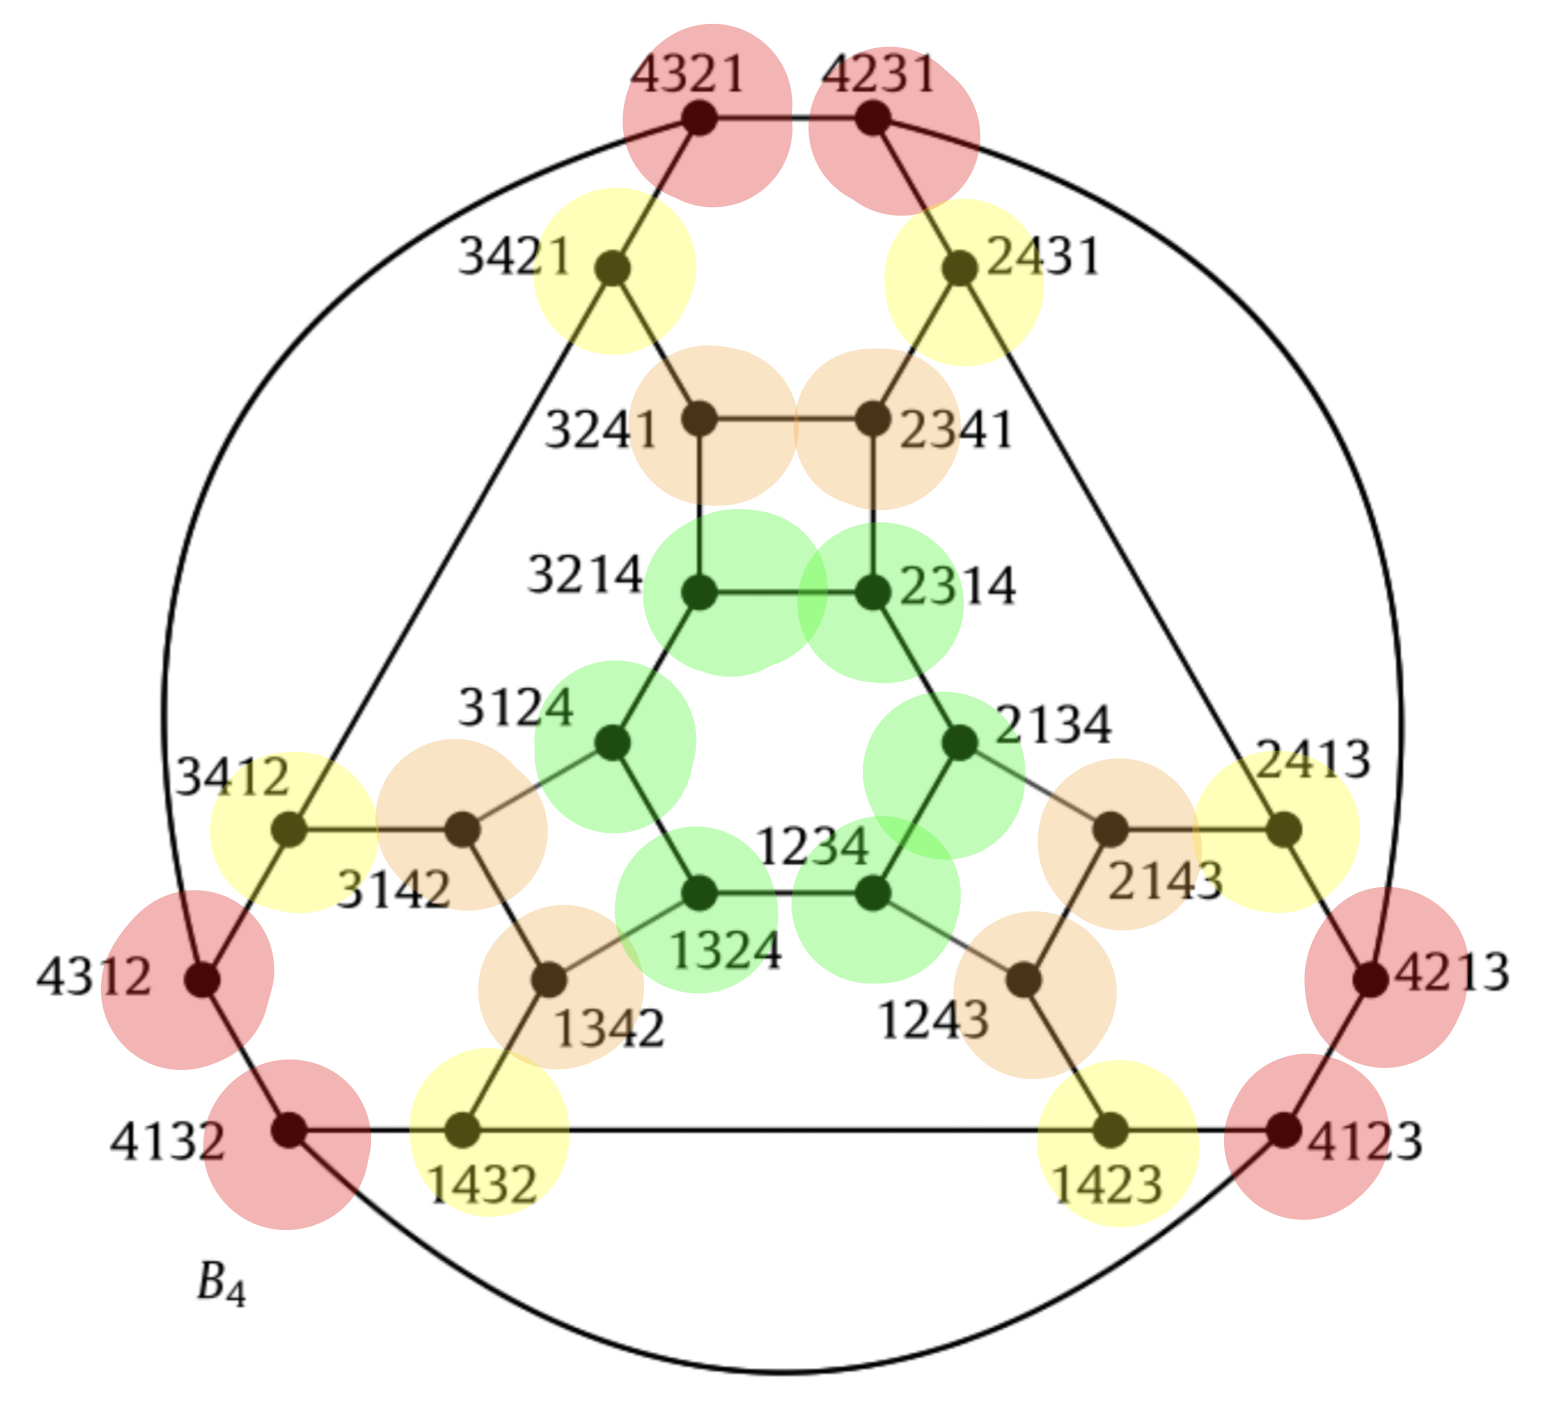
\includegraphics[width=0.6\textwidth]{ans-4.png}
      \end{center}
      We now consider the algebraically-defined automorphism (we will prove that this is an automorphism):
      \begin{align*}
        \sigma: V &\to V \\ 
        \sigma(a_1, a_2, a_3, a_4) &= ((a_1 \bmod 4) + 1, (a_2 \bmod 4) + 1, (a_3 \bmod 4) + 1, (a_4 \bmod 4) + 1).
      \end{align*}
      $\sigma$ is an automorphism if it is a permutation and is channel-preserving. We let $\bm a = (a_1, a_2, a_3, a_4), \bm b = (b_1, b_2, b_3, b_4) \in V$ be distinct nodes of $B_4$. Suppose that $\sigma(\bm a) = \sigma(\bm b)$. But then
      \[ (a_2, a_1, a_3, a_4) = (b_2, b_1, b_3, b_4); \]
      that is, $\bm a = \bm b$; a contradiction as $\bm a$ and $\bm b$ were assumed to be distinct. Thus $\sigma$ indeed defines a permutation. Now we consider $\bm a = (a_1, a_2, a_3, \ldots, a_4) \in V$ and its neighbours:
      \[ (a_2, a_1, a_3, a_4), (a_1, a_3, a_2, a_4), (a_1, a_2, a_4, a_3) \in E. \]
      We let $\sigma(\bm a) = (b_1, b_2, b_3, b_4) \in V$ and consider the image of the edges from $\bm a$.
      \begin{align*}
        (\sigma(\bm a), \sigma(a_2, a_1, a_3, a_4)) &= (\bm b, (b_2, b_1, b_3, b_4)) \in E, \\
        (\sigma(\bm a), \sigma(a_1, a_3, a_2, a_4)) &= (\bm b, (b_1, b_3, b_2, b_4)) \in E, \\
        (\sigma(\bm a), \sigma(a_1, a_2, a_4, a_3)) &= (\bm b, (b_1, b_2, b_4, b_3)) \in E.
      \end{align*}
      These edges are contained within $E$ as $\sigma: V \to V$ is bijective and each endpoint in the edges can be obtained by flipping adjacent numbers in the other endpoint in the edge. 
      Thus for every vertex its edges are all preserved; thus $\sigma$ is channel preserving and thus an automorphism.

      We now claim that appropriate compositions of the three introduced automorphisms (and their inverses) are adequate in showing that $B_4$ is node-symmetric. First, we note that the composition of two automorphisms also defines an automorphism and that the inverse of an automorphism is also an automorphism. From the earlier image, we have the following \emph{classes} in which we can construct an automorphism between any two nodes of the same class:
      \begin{align*}
        C_1 &= \{(4,3,2,1), (4,3,1,2), (4,1,3,2), (4,1,2,3), (4,2,1,3), (4,2,3,1)\}, \\
        C_2 &= \{(3,4,2,1), (3,4,1,2), (1,4,3,2), (1,4,2,3), (2,4,1,3), (2,4,3,1)\}, \\
        C_3 &= \{(3,2,4,1), (3,1,4,2), (1,3,4,2), (1,2,4,3), (2,1,4,3), (2,3,4,1)\}, \\
        C_4 &= \{(3,2,1,4), (3,1,2,4), (1,3,2,4), (1,2,3,4), (2,1,3,4), (2,3,1,4)\}.
      \end{align*}
      Using $\sigma$, we can connect these classes together. Indeed, consider the following:
      \begin{align}
        \sigma(4,3,2,1) &= (1,4,3,2), \\
        \sigma(1,4,3,2) &= (2,1,4,3), \\
        \sigma(4,2,1,3) &= (1,3,2,4).
      \end{align}
      We see that $(1)$ connects $C_1$ to $C_2$, $(2)$ connects $C_2$ and $C_3$, and $(3)$ connects $C_1$ and $C_4$. Thus, we have shown that using composition of the two geometric automorphisms and $\sigma$ (as well as their inverses), we can construct an automorphism between any two nodes of the graph. 
    \end{solution}
  \end{parts}
  \begin{figure}
      \centering
      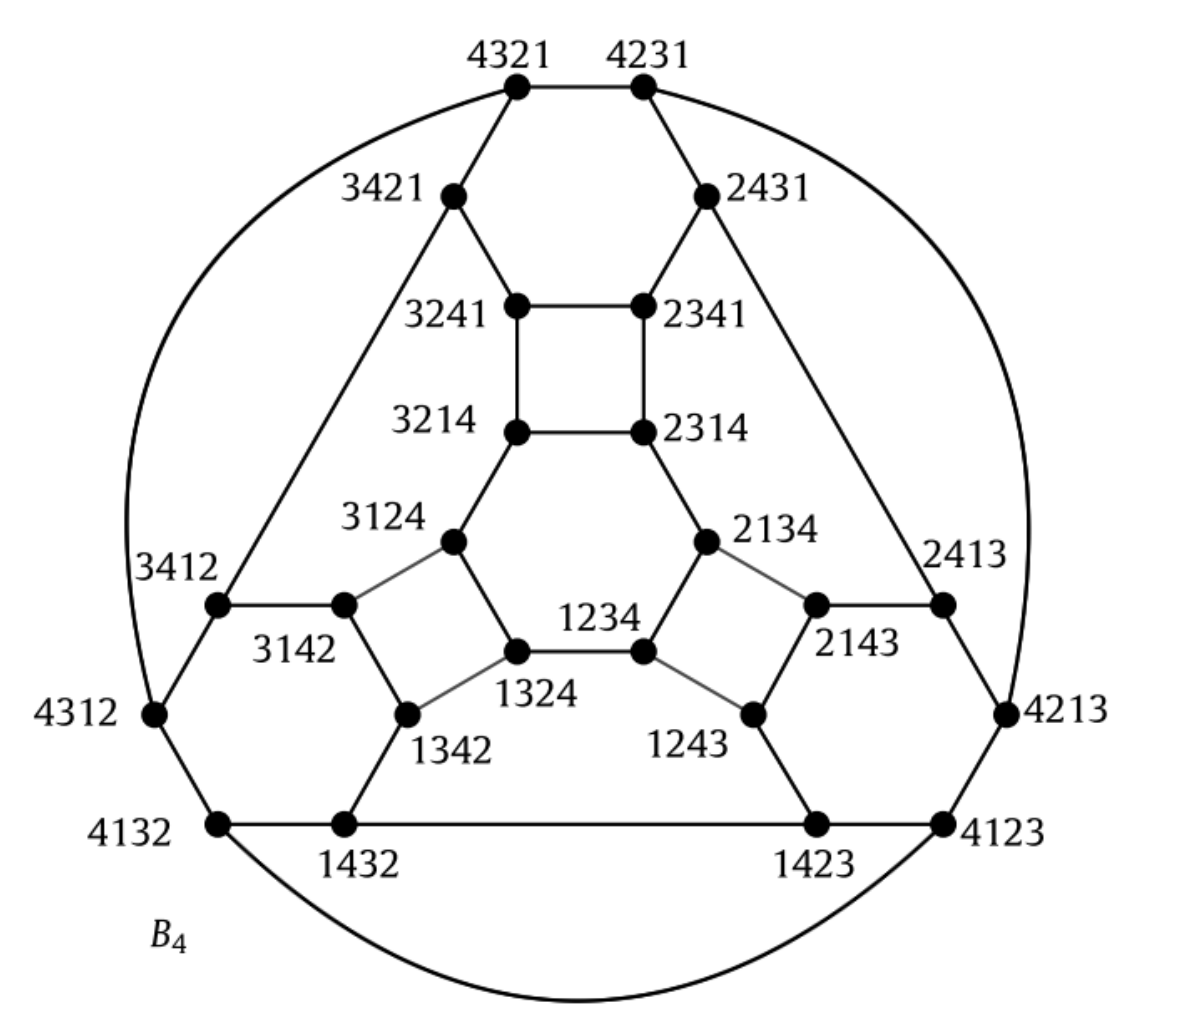
\includegraphics[width=0.5\textwidth]{fig-2}
      \caption{The bubble-sort interconnection network $B_4$.}
  \end{figure}

  \question Consider a supercomputer $\mathcal K$ whose interconnection network is a $4$-ary $3$-cube $Q_3^4$ whose node set is $\{(u_1, u_2, u_3): 0 \leq u_1, u_2, u_3 \leq 3\}$ and whose edge set is
  \begin{align*}
    \{
      ((u_1, u_2, u_3), (v_1, v_2, v_3)):
        &\; 0 \leq u_1, u_2, u_3, v_1, v_2, v_3 \leq 3, \\
        &\; v_1 = u_1 \pm 1, u_2 = v_2, u_3 = v_3 \;\;\text{or} \\
        &\; v_1 = u_1, u_2 = v_2 \pm 1, u_3 = v_3 \;\;\text{or} \\
        &\; v_1 = u_1, u_2 = v_2, u_3 = v_3 \pm 1 \;\text{with addition modulo $4$}
    \}.
  \end{align*}
  Suppose, for simplicity, that $\mathcal K$ operates synchronously in that there is a global clock and at each tick of the click: some computation is undertaken by every node (the computation phase); at most one new message is generated for each of the neighbours of a node (the generation phase); and at most one message is sent to each neighbour of a node (the message phase). Of course, a node might receive messages, in the message phase, from neighbours that are intended for other nodes and that need to be passed on in an upcoming message phase. Every message includes in its header the full route of that message and so any node can immediately detect the neighbour to which the message is to be sent. For every output channel, there is a buffer that holds the messages that need to be sent down the channel in an upcoming message phase to the corresponding neighbour and any generated or received message is automatically placed in the correct buffer (at the end of the corresponding generation or message phase, respectively). All messages have size one unit and buffer sizes are measured in units.

  There is a Hamiltonian cycle $H$ in $Q_3^4$ defined as follows:
  \begin{align*}
    &(0, 0, 0), (1, 0, 0), (2, 0, 0), (3, 0, 0), (3, 1, 0), (2, 1, 0), (1, 1, 0), (0, 1, 0), \\
    &(0, 2, 0), (1, 2, 0), (2, 2, 0), (3, 2, 0), (3, 3, 0), (2, 3, 0), (1, 3, 0), (0, 3, 0), \\
    &(0, 3, 1), (1, 3, 1), (2, 3, 1), (3, 3, 1), (3, 2, 1), (2, 2, 1), (1, 2, 1), (0, 2, 1), \\
    &(0, 1, 1), (1, 1, 1), (2, 1, 1), (3, 1, 1), (3, 0, 1), (2, 0, 1), (1, 0, 1), (0, 0, 1), \\
    &(0, 0, 2), (1, 0, 2), (2, 0, 2), (3, 0, 2), (3, 1, 2), (2, 1, 2), (1, 1, 2), (0, 1, 2), \\
    &(0, 2, 2), (1, 2, 2), (2, 2, 2), (3, 2, 2), (3, 3, 2), (2, 3, 2), (1, 3, 2), (0, 3, 2), \\
    &(0, 3, 3), (1, 3, 3), (2, 3, 3), (3, 3, 3), (3, 2, 3), (2, 2, 3), (1, 2, 3), (0, 2, 3), \\
    &(0, 1, 3), (1, 1, 3), (2, 1, 3), (3, 1, 3), (3, 0, 3), (2, 0, 3), (1, 0, 3), (0, 0, 3), (0, 0, 0).
  \end{align*}
  \begin{parts}
    \part Explain how we can use $H$ to undertake a single-node scatter from $(0,0,0)$ in $\mathcal K$ (as in slide 8 of Lecture 4). Be sure to detail the number of clock-ticks required and the maximal size of any channel buffer.
    \begin{solution}
      Let $n_i$ denote the $i$th node in the Hamiltonian cycle $H$ ($n_0 = (0,0,0)$).
      On the first clock cycle, we generate the message intended for $n_{63} = (0,0,3)$. 
      Then on the $k$th clock cycle ($k \in \{2, 3, \ldots, 63\}$), we generate the message for node $n_{64 - k}$ and send the message for node $n_{64-k+1}$ (which is generated in the $(k-1)$th clock cycle). Then on the $64$th clock cycle, we send the message to $(1,0,0)$ (which was generated on the $63$rd clock cycle). Thus, by the end of the $64$th cycle all nodes have received their message. This requires a maximal buffer size of 1 and 64 clock cycles until all nodes have received their message. 
    \end{solution}

    \part There is another supercomputer $\mathcal Q$ where the interconnection network is the $3$-dimensional hypercube $Q_3$. We wish to simulate the single-node scatter of $\mathcal K$ in $\mathcal Q$. Explain how we might do this and comment on the overheads arising from your simulation. 
    \begin{solution}
      We describe an embedding from $\mathcal K$ to $\mathcal Q$: the first 8 nodes of the Hamiltonian cycle $H$ is mapped to $(0,0,0)$. The next 8 nodes are mapped to $(1,0,0)$ and so on. Then we proceed with the simulation by timesharing each of the virtual processors that are mapped to each node of $\mathcal Q$. If $\varphi$ is the embedding we described above, if a message was to be sent between $x$ and $y$ in $\mathcal K$ it is instead sent between $\varphi(x)$ and $\varphi(y)$ (in the case that $\varphi(x) = \varphi(y)$, we place this message in the buffer). This embedding has a load of $8$, congestion $8$, and dilation $1$ and will require a buffer of $8$ at each node of $\mathcal Q$.
      % Firstly, we are going to construct an embedding from $Q_3^4$ to $Q_3$ to help motivate the simulation. 
      % Consider $Q_3$ where
      % \begin{align*}
      %   V(Q_3) &= \Z/2 \oplus \Z/2 \oplus \Z/2, \\
      %   E(Q_3) &= \{((\overline u_1, \overline u_2, \overline u_3), (\overline{u_1 + 1},\overline u_2,\overline u_3)): \overline u_1, \overline u_2, \overline u_3 \in \Z/2\} \;\cup \\
      %   &\qquad \{((\overline u_1, \overline u_2, \overline u_3), (\overline u_1,\overline{u_2+1},\overline u_3)): \overline u_1, \overline u_2, \overline u_3 \in \Z/2\} \;\cup 
      %   \\ &\qquad \{((\overline u_1, \overline u_2, \overline u_3), (\overline u_1,\overline u_2,\overline{u_3+1})): \overline u_1, \overline u_2, \overline u_3 \in \Z/2\}.
      % \end{align*}
      % To make the construction of our embedding clear, we will consider $Q^4_3 = \left(V(Q^4_3), E(Q^4_3)\right)$ where $V(Q^4_3) = \Z/4 \oplus \Z/4 \oplus \Z/4$ and $E(Q^4_3)$ is defined as in the statement of the question.
    \end{solution}
  \end{parts}

  \question Suppose you have a supercomputer $\mathcal C$ whose interconnection network is the $3$-dimensional hypercube $Q_3$. However, you have a fault-tolerant software application $S$ that never terminates, is designed for a supercomputer $\mathcal D$ whose interconnection network is $Q_4$ and can tolerate one faulty processor.
  \begin{parts}
    \part Explain how you might make use of an embedding to run $S$ on $\mathcal C$ and describe any overheads accruing.
    \begin{solution}
      We consider $V(Q_4) = \{0,1\}^4$ and $V(Q_3) = \{0,1\}^3$. With our embedding, we still want our software to be fault tolerant. However, if we have multiple nodes (in the guest network) mapped to a single node (in the host network), then a failure of this node will cause the software to be unable to run, as we can only deal with a single faulty processor. To mitigate this, we can maximise the number of one-to-one mappings in our embedding. By doing this, we may get an embedding $\varphi$ like the following:
      \begin{align*}
        (a_1, a_2, a_3, 0) &\mapsto (0, 0, 0), \\
        (a_1, a_2, a_3, 1) &\mapsto (a_1, a_2, a_3)
      \end{align*}
      for all $a_1, a_2, a_3 \in \{0,1\}$. Lets describe how the channels may get mapped, here we are trying to map channels to paths such as to minimise the congestion. 
      \begin{enumerate}
        \item Edges of the form $((a_1,a_2,a_3,1), (b_1, b_2, b_3, 1))$ get mapped to $((a_1,a_2,a_3),(b_1,b_2,b_3))$.
        \item Edges of the form $((a_1, a_2, a_3, 0), (b_1,b_2,b_3,0))$ get mapped to the empty path (as they get contracted into $(0,0,0)$).
        \item The edge $((0,0,0,0), (0,0,0,1))$ also gets mapped to the empty path as it is also contracted into $(0,0,0)$.
        \item Finally, we need to pick a suitable mapping for edges of the form 
        \[ ((a_1,a_2,a_3,0), (a_1, a_2, a_3, 1)) \]
        (excluding the case in (iii)). Observe that $\varphi(a_1,a_2,a_3,0) = (0,0,0)$ and $\varphi(a_1,a_2,a_3,1) = (a_1,a_2,a_3)$. So we are looking paths from $(0,0,0)$ to every other point in $Q_3$ that minimises congestion and dilation. We observe that, in $Q_3$, $(0,0,0)$ has 3 outgoing channels, thus as we have 7 paths to form, the congestion must be at least 3. Furthermore, the shortest path from $(0,0,0)$ to $(1,1,1)$ is 3, and so the dilation must be at least $3$. We can indeed attain both of these minimums with the following assignments.
        {\small
          \begin{align*}
            ((1,0,0,0), (1,0,0,1)) &\mapsto ((0,0,0), (1,0,0)), \\
            ((0,1,0,0), (0,1,0,1)) &\mapsto ((0,0,0), (0,1,0)), \\
            ((0,0,1,0), (0,0,1,1)) &\mapsto ((0,0,0), (0,0,1)) \\
            ((1,1,0,0), (1,1,0,1)) &\mapsto ((0,0,0), (1,0,0), (1,1,0)), \\
            ((1,0,1,0), (1,0,1,1)) &\mapsto ((0,0,0), (0,0,1), (1,0,1)), \\
            ((0,1,1,0), (0,1,1,1)) &\mapsto ((0,0,0), (0,1,0), (0,1,1)), \\
            ((1,1,1,0), (1,1,1,1)) &\mapsto ((0,0,0), (1,0,0), (1,1,0), (1,1,1)). 
          \end{align*}
        }
        I have displayed the graphically below.
        \begin{center}
          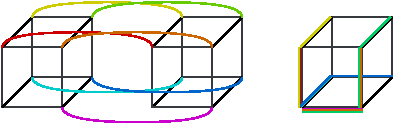
\includegraphics{q6-embedding.pdf}
        \end{center}
        It is clear to see that our load is 9, our congestion is 3, and our dilation is also 3. 
      \end{enumerate}
      To run $S$ on $\mathcal C$, for each processor $p \in \{0,1\}^3$ of $\mathcal C$, we simulate each processor in $\varphi^{-1}(\{p\})$; that is, each processor mapped to $p$. This can be done by time-sharing, and if a message is originally sent along the channel $(x,y)$ in $Q_4$, it is instead sent along the described path from $\varphi(x)$ to $\varphi(y)$ which is described above. In this situation, the simulation requires significant buffer space as 9 processors have been mapped to a single processor. So any messages being sent between these 9 nodes will have to be stored in a buffer. The reason for the high load is to ensure that the program is still fault tolerant. One may argue that increasing the load on processor $(0,0,0)$ to 9 times its original load may cause it to be more likely to fail, but it may be the case that the expected chance of failure is still lower than in the situation where we may spread our mapping more evenly throughout $Q_3$. 
    \end{solution}

    \part Suppose that from time to time you obtain the resources to buy an additional processor. Explain how you might incrementally scale $\mathcal C$ by incorporating these processors one at a time and so that there is never any need to pause the execution of $S$.

    [You may assume that you have access to an unlimited supply of processor-to-processor cables.]
    \begin{solution}
      We can utilise the fault-tolerance of $S$ to upgrade $\mathcal C$ without causing a pause in execution. There would be no need to expand $\mathcal C$ past the size of the original interconnection network, so we assume we have $k \in \{8, \ldots, 15\}$ processors (think of this as the step number) and we wish to add a $(k+1)$th processor. Consider the following path (in $Q_4$):
      \[ P = ((0,0,0,0), (1,0,0,0), (1,1,0,0), (0,1,0,0), (0,1,1,0), (1,1,1,0), (1,0,1,0), (0,0,1,0)) \]
      and let $P_i$ denote the $i$th entry in $P$ ($P_1 = (0,0,0,0)$). To add this $(k+1)$th processor, we disable the (logical) processor $P_{k-7}$ (which is currently being mapped to node $(0,0,0)$). As $S$ is fault-tolerant, it can handle this processor being disabled. We then add our $(k+1)$th processor to our network, joining it to $(0,0,0)$ and also to every other processor we have added beyond $Q_3$ (i.e. the processors added in step $8, 9, \ldots, k-1$). By doing this, we remove all previous mappings we had in our embedding for $P_{k-7}$. The only changes to software which would be needed is in the routing tables at $(0,0,0)$. All other nodes should route to nodes mapped to $(0,0,0)$ as normal, but as $(0,0,0)$ is either adjacent to one of the nodes that were originally mapped to it or is itself simulating that node then it can either place it in the internal buffer, or directly send it to the new node added for said node. To discuss the overheads here, we would indeed have a large number of processor-to-processor cables as we are effectively building a complete graph off of a single node in $Q_3$. Our load would decrease by 1 for every node we add, our congestion we remain constant, and our dilation would increase to 4 after the first processor addition, but stay constant with further additions. 
    \end{solution}
  \end{parts}
